\section{Mapping Discordant Features}\label{sec:mapping}

In this section, I first map the spatial distribution of topographic discordance at the summit of Olympus Mons and define candidate axisymmetric inflation center locations to explain this discordance. Next, I begin the process of translating discordance into tilt-distance datasets for comparison with solutions from Section~\ref{sec:modeling}. For each sampled location at the surface, both tilt and distance depend on the horizontal position of the axisymmetric inflation center. Since I don't know where this center is, I construct a large spatial array of candidate center points to test. For each pair of points (one center candidate and one discordant sample location) I calculate the tilt necessary to explain the discordance of the sample location about the horizontal axis imposed by the chosen center candidate. This results in a tilt-distance dataset for each center candidate (and for each population of discordant features evaluated).

\subsection{Attitude Data from Discordant Features}\label{sec:attitude-data}

I use the \ac{CTX} mosaic to visually identify lava flows in the study area. Following \textcite{mouginis-mark_geologic_2021}, I map lobate flow outlines as polygons where possible. From these polygons, I derive centerline features using the \hlss{Polygon To Centerline} tool in ArcGIS Pro, as shown in Figure~\ref{fig:linear-features}. Where flow margins are not visible, I map lava channels directly as linear features. I include discontinuous regions where I infer partial collapse of lava tubes yielding skylight chains,\footnote{This assumption of underlying continuity follows, e.g., \textcite{bleacher_olympus_2007,carr_geologic_2010,peters_lava_2021}.} as shown in Figure~\ref{fig:linear-features}.

While I maintain a consistent ``sense'' in mapping channels (pointing \emph{away} from the caldera complex), the \hlss{Polygon To Centerline} tool does not. I use the \hlss{Flip Line} tool to reverse the orientation of any features pointing in the paleo-uphill direction. Then I use the \hlss{Calculate Geometry Attributes} tool to find the average azimuthal orientation for each linear feature. This result defines \acf{az1} for each centerline (``flowpath'') and channel.

\newcommand{\samplinginterval}{\qty{3}{\km}}

Along each feature, I use the \hlss{Generate Points Along Line} tool with sampling interval \samplinginterval\ to create a series of point features for further attitude data collection and analysis. Note that features shorter than $<\samplinginterval$ are not sampled at all on the grounds that they are unlikely to accurately record regional paleo-topographic downhill azimuth.

I use a point-based sampling approach for a few reasons. First, modern topographic attitude can be measured to high precision using the \ac{MOLA} \ac{DEM} and may vary across the length of lava features, so a single value is not appropriate.\footnote{\Acf{az1} is much less certain since lava does not always flow exactly in the regional downhill direction.} More importantly, the analysis described later in Section~\ref{sec:tilt-from-map} is extremely sensitive to position---different locations even with identical paleo- and modern attitude can imply vastly different tilt and distance relative to an axisymmetric inflation center. Finally, discrete points are necessary for the tilt-distance regression analysis in Section~\ref{sec:evaluation}.

\begin{figure}
    \includegraphics[width=\textwidth]{methods/linear-features.pdf}
    \includegraphics[width=\textwidth]{methods/linear-features-mapped.pdf}
    \caption[Mapping linear features]{\textbf{Top:} Lobate flows and linear channel features identified from the \acs{CTX} basemap. \textbf{Bottom:} Point samples derived along the linear channel and lobate flow centerlines.}%
    \label{fig:linear-features}
\end{figure}

\newcommand{\neighborhood}{\qty{2}{\km}}

I collect three attitude variables for each sampled point. \Acf{az1} is inherited from the parent linear feature as described above. Since \ac{az1} is defined but \acf{sl1} is unknown, the implied paleo-surface attitude is actually a \emph{family} of possible attitudes. The corresponding graphical representation (from Section~\ref{sec:attitude-representation}) is thus a line of poles rather than a single pole.

For the modern surface attitude, I use the \hlss{Surface Parameters} tool on the \ac{MOLA} \ac{DEM} to compute average topographic \hlss{Slope} and \hlss{Aspect} (downhill azimuth) rasters across the entire study area. To avoid capturing local topographic anomalies, these values are averaged over a ``neighborhood'' with radius \neighborhood. I use the \hlss{Extract Multi Values to Points} tool to assign \ac{sl2} and \ac{az2} to each sample point based on the value of the corresponding raster value at that location. Unlike the paleo-attitude, the modern attitude is fully defined by a single pole in attitude space, as in Figure~\ref{fig:surface}. Figure~\ref{fig:attitude-data} illustrates an example dataset collected for a single point.

\begin{figure}
    \floatbox[{\capbeside\thisfloatsetup{floatwidth=sidefil,capbesideposition={left,center},capbesidewidth=.7\linewidth}}]{figure}
    {\caption[Sample point attitude dataset]{
        Example dataset associated with a single point sampled from a discordant feature. The line labeled \acs{az1} represents the family of paleo-attitudes consistent with a mapped feature pointing downhill in the same direction as the arrow. The point labeled $(\acs{az2},\acs{sl2})$ represents the modern attitude based on \ac{MOLA} topography.
    }\label{fig:attitude-data}}
    {\begin{tikzpicture}[scale=.7]

    \coordinate (orig) at (0,0);
    \coordinate (s2) at (-60:1);

    %\draw[green!70!black,ultra thick] (s2) + (83:.3) arc (83:120:.3);

    \draw (orig) circle (\flatradius);

    \draw[arrow, ultra thick] (orig) -- (70:\flatradius) node[anchor=south] {\acs{az1}};
    \fill (s2) circle (1mm) node[anchor=north] {$(\acs{az2},\acs{sl2})$};

    %\draw[] (s2) -- (orig);
    %\draw[] (s2) -- (70:\flatradius);


\end{tikzpicture}%}
\end{figure}

These measurements (\acf{az1}, \acf{az2}, and \acf{sl2}) for each sample point constitute the first intermediate product of this section. In particular, I calculate \acl{disc} as the difference between the modern and paleo- downhill azimuths. To express \ac{disc} in the range \ang{-180} to \ang{180}, I use the explicit equation:
\begin{equation}
    \acs{disc} = ([\acs{az2} - \acs{az1} + \ang{180}] \text{ mod } \ang{360}) - 180.
\end{equation}

Using this calculation I identify regions of highly discordant flows to target for matching with tilt solutions from Section~\ref{sec:modeling}. From preliminary analysis I suspect many discordant features will cluster closely around the caldera rim, recoding proximal collapse effects. % PUT STUFF HERE ABOUT WHAT THOSE EFFECTS ARE 
For assessing elastic response, I thus focus on discordant regions away from the rim.

\subsection{Tilt-Distance Datasets from Attitude Data}\label{sec:tilt-from-map}

In this section I translate mapped attitude data from Section~\ref{sec:attitude-data} into tilt-distance datasets for direct comparison with the solutions from Section~\ref{sec:modeling}. After showing why this dataset construction depends on the (unknown) position of the axisymmetric center, I define a spatial grid of candidate center points to evaluate. Next, I convert position and attitude data for a sample point into distance and tilt relative to a particular candidate center. I repeat this conversion for each sample (within a discordant population of interest) to produce a tilt-distance dataset corresponding to one center candidate. Finally, I repeat the full tilt-distance dataset generation for each center candidate.

\subsubsection{Axisymmetric Center Candidates}

In Section~\ref{sec:modeling}, the particular center location plays only a limited role in the model analysis. In the numerical solution (Section~\ref{sec:numerical-tilt-solution}) this position reproduces the large-scale topography of Olympus Mons to first order. However, the edifice topography minimally influences surface tilt resulting from subsurface pressure change (Figure~\ref{fig:grav-topo-test}). The analytical model (Section~\ref{sec:analytical-tilt-solution}) eliminates dependence on center position (within the edifice) altogether by treating the host rock as a flat infinite half-space.

However, fitting a particular spatial distribution of attitude data into this framework requires a particular center point. Expressing the coordinates of mapped features as a distance from a center point clearly depends on the location of that center point. Less obviously, the choice of center position also determines the amount of tilt necessary to account for a topographically discordant feature by imposing a particular \emph{axis of tilt}. Since all displacement in an axisymmetric model is confined to a vertical cross-section, rotation (tilt) can only occur about the axis perpendicular to the vertical cross-sectional plane (the white surface in Figure~\ref{fig:axisymmetry}). This tilt axis is horizontal and perpendicular to the line from sample point to center. Importantly, the magnitude of surface tilt implied by a discordant sample depends on the orientation of the tilt axis. The role of center point location in calculating both tilt and distance for a particular sample point is illustrated schematically in Figure~\ref{fig:center-significance}.

\begin{figure}
    \begin{tikzpicture}[scale=1]
    
    % origin
    \coordinate (c1) at (0,0);
    \coordinate (c2) at (9,3);
    
    \coordinate (s1) at (3,3);
    
    \draw[red, thick] (s1) + (-45:1) --+ (135:1);
    \draw[blue, thick] (s1) + (-90:1) --+ (90:1);

    \draw[thick, -latex, rotate around={90:(s1)}] (s1) + (8 mm,0) arc (0:360:1 mm and 3 mm);
    
    \draw[thick, -latex, rotate around={-45:(s1)}] (s1) + (8 mm,0) arc (0:360:1 mm and 3 mm);
    
    \draw[white, line width = 1 mm] (s1) --+ (-45:0.65);
    \draw[white, line width = 1 mm] (s1) --+ (90:0.65);
    \draw[red, thick] (s1) --+ (-45:0.7);
    \draw[blue, thick] (s1) --+ (90:0.7);
    
    
    \fill[red] (c1) circle (1mm) node[anchor = north east] {$C_1$};
    \fill[blue] (c2) circle (1mm) node[anchor = south] {$C_2$};
    
    \draw[red, dashed, thick] (c1) -- node[sloped, fill=white] {$\acs{dist}_{C_1}$} (s1);
    \draw[blue, dashed, thick] (c2) -- node[fill=white] {$\acs{dist}_{C_2}$} (s1);
    
    \fill (s1) circle (1mm) node[anchor = south west] {$S$};

\end{tikzpicture}%
    \caption[Significance of center position for tilt, distance calculations]{Schematic map view illustrating the role of inflation center position in expressing a discordant sample point ($S$) in terms of distance and tilt. Clearly, different center points ($C_1, C_2$) are different distances ($\acs{dist}_{C_1},\acs{dist}_{C_2}$) from the sample. More subtly, the azimuth orientation of each center imposes a different tilt axis (solid colored line), which influences the subsequent tilt calculation.}%
    \label{fig:center-significance}
\end{figure}

However, the position of magma reservoir(s) within/below the Olympus Mons edifice is one of the central unanswered questions driving this thesis. Since inflation center position controls the magnitude of surface tilt implied by discordant features, it is worth assessing the plausibility of a wide range of potential inflation centers.

To define this array of inflation center candidates, I use the \hlss{Generate Tesselation} and \hlss{Feature to Point} tools in ArcGIS Pro to generate an evenly spaced array in the caldera vicinity as shown in Figure~\ref{fig:candidates}. This array includes the caldera and southern summit bulge, the two regions I suspect to be most responsible for discordant features. Each of 781 points is less than \qty{4}{\km} from its six neighbors to ensure spatial resolution similar to the sampling interval (\samplinginterval) for \acl{az1} and modern topographic ``neighborhood'' (\neighborhood) for modern attitude measurements, without creating unnecessary computational expense.

\begin{figure}
    \includegraphics[width=\textwidth]{methods/candidates.pdf}%
    \caption{Axisymmetric center location candidates}%
    \label{fig:candidates}
\end{figure}

\subsubsection{Spatial Description of Samples}

In this section I express the position of a sample point by its distance (\acs{dist}) and azimuth angle (\acs{bearing}) \emph{away} from a center candidate. The former is used directly in constructing the tilt-distance dataset; the latter is necessary to define an axis for calculating tilt. These calculations quantify the key spatial relationships introduced in Figure~\ref{fig:center-significance}.

To calculate distance (\acs{dist}), I use the spherical law of cosines\footnote{Also known as the great circle distance formula, derived in Appendix~\ref{app:gcd}.} scaled by the martian equatorial radius since Olympus Mons is close to the equator:
\begin{equation}
    \acs{dist}=\arccos(\cos\acs{latC}\cos\acs{lat}\cos(\acs{lonC}-\acs{lon}) + \sin\acs{latC}\sin\acs{lat})\cdot\qty{3396.2}{\km},\label{eq:dist}
\end{equation}
where \acs{latC} and \acs{lonC} are the latitude and longitude of the center; \acs{lat} and \acs{lon} are the latitude and longitude of the sample.

To calculate the azimuth angle from a sample directly \emph{away}\footnote{This ensures the horizontal \acs{bearing}-axis points in the same direction as increasing \acs{dist}.} from the center (\acs{bearing}),\footnote{This value is different from the azimuth from the center to the sample, although they represent the same physical direction.} I use the following equation from \textcite{williams_aviation, veness_calculate}:
\begin{equation}
    \acs{bearing} = \ang{180} + \arctan\left(\frac{\sin(\acs{lonC}-\acs{lon})\cos\acs{latC}} {\cos\acs{lat} \sin\acs{latC}-\sin\acs{lat}\cos\acs{latC}\cos(\acs{lonC}-\acs{lon})}\right).\label{eq:bearing}
\end{equation} 

\subsubsection{Paleo-Slope Equation}\label{sec:paleo-slope}

\begin{figure}
\begin{center}
    \begin{tikzpicture}[scale=5,tdplot_main_coords]
    % origin
    \coordinate (orig) at (0,0,0);
    
    % also defines (Pxy), (Pxz), (Pyz), etc.
    \tdplotsetcoord{P}{\radius}{\ze}{\az}
    \tdplotsetcoord{C}{-0.4*\axislength}{90}{\THETA}
    \tdplotsetcoord{P'}{\radius}{\zen}{\azi}
    \tdplotsetcoord{tiltintercept}{\deltalength}{90}{\THETA-90}
    \tdplotsetcoord{rintercept}{0.68}{90}{\THETA}
    
    % gray rectangle
    \fill[tdplot_main_coords, color = gray!30!white] (orig) -- (tiltintercept) -- (Pxy) -- (rintercept);
    \draw[tdplot_main_coords] (\THETA-90:\radius) arc (\THETA-90:\THETA:\radius);

    % z-axis
    \draw[arrow] (orig) -- (0,0,\axislength) node[anchor=south]{$z$};
    \draw[arrow] (orig) -- (\THETA:\axislength) node[anchor=north east]{$r$};
    \draw[arrow] (orig) -- node[sloped, fill=white, pos=.65]{Tilt Axis} (\THETA-90:\axislength);

    % az' surface
    \tdplotsetthetaplanecoords{\azi}

    \draw[tdplot_rotated_coords] (90:\radius) -- (0,0.76604444*\radius) -- (0,0);
    \tdplotdrawarc[tdplot_rotated_coords, line width = 1mm]{(orig)}{\radius}{0}{90}{anchor=east}{\acs{az1}}

    % \draw[very thin, dashed] (P') -- (P'xy) -- (orig);
    % \draw (orig) -- (P');

    % surface vertical from axis
    \tdplotsetthetaplanecoords{\THETA+90}

    % proj1 line
    \tdplotdrawarc[tdplot_rotated_coords]{(orig)}{\radius}{-90}{0}{}{}
    
    % r-z surface, fill, line
    \tdplotsetthetaplanecoords{\THETA}
    % \fill[tdplot_rotated_coords, color = red, opacity = 0.1] (\zenproj:\radius) arc (\zenproj:\zeproj:\radius) -- (0,0);     
    \tdplotdrawarc[arrow, tdplot_rotated_coords]{(orig)}{\radius}{0}{90}{}{}
    \tdplotdrawarc[arrow, tdplot_rotated_coords,red,line width=1mm]{(orig)}{\radius}{\zenproj}{\zeproj}{anchor=south west}{\textcolor{black}{\acs{tilt}}}

    % az2 surface
    \tdplotsetthetaplanecoords{\az}
    \draw[very thin, dashed] (P) -- (Pxy) -- (orig);
    % \draw (orig) -- (P);
    
    % az angle labels
    %\tdplotdrawarc{(orig)}{0.33}{\THETA}{\azi}{}{}%{fill=white, anchor=south east}{\acs{beta1}}
    %\tdplotdrawarc{(orig)}{0.37}{\THETA}{\az}{}{}%{anchor=north west}{\acs{beta2}}

    % translate THETA surface to small circle
    \tdplotsetthetaplanecoords{\THETA}
    \tdplotsetrotatedcoordsorigin{(tiltintercept)}
    \draw[tdplot_rotated_coords] (0:\smallcircleradius) arc (0:90:\smallcircleradius) -- (0,0.76604444*\smallcircleradius) -- (0,0) -- cycle;
    \tdplotdrawarc[arrow, tdplot_rotated_coords]{(tiltintercept)}{\smallcircleradius}{\zenproj}{\zeproj}{coordinate}{}
    
    % translate THETA surface to back to great circle
    \tdplotsetrotatedcoordsorigin{(orig)}

    % proj1 plane, line, fill
    \tdplotsetrotatedcoords{\THETA}{-90+\zenproj}{0}
    \tdplotdrawarc[tdplot_rotated_coords, blue, ultra thick]{(0,0,0)}{\radius}{\asindelta}{0}{}{}
    \fill[tdplot_rotated_coords, color = blue, opacity = 0.2] (\asindelta:\radius) arc (\asindelta:0:\radius) -- (0,0) -- (tiltintercept);

    % proj2 plane, fill, line,
    \tdplotsetrotatedcoords{\THETA}{-90+\zeproj}{0}
    \fill[tdplot_rotated_coords, color = green!70!black, opacity = 0.3] (\asindelta:\radius) arc (\asindelta:0:\radius) -- (0,0) -- (tiltintercept);
    \tdplotdrawarc[tdplot_rotated_coords, green!70!black, ultra thick]{(0,0,0)}{\radius}{\asindelta}{0}{}{}
    
    % (az2, sl2) point
    \fill (P) circle (0.2mm) node[anchor = north east] {$(\acs{az2},\acs{sl2})$};
\end{tikzpicture}%
\hspace{1cm}%
\newcommand{\dotradius}{.3pt}%
\begin{tikzpicture}[scale=8]%
    \coordinate (orig) at (0,0);

    \coordinate (tiltintercept) at (\deltalength,0);
    \coordinate (pole1) at (\deltalength,\poleoneflatx);
    \coordinate (pole2) at (\deltalength,\poletwoflatx);
    \coordinate (rendpoint) at (0,\poletwoflatx+0.2);
    \coordinate (rintercept2) at (0,\poletwoflatx);    
    \coordinate (rintercept1) at (0,\poleoneflatx);    

    \coordinate (tiltaxisendpoint) at (\deltalength,0);
    
    \draw[dashed] (rintercept2) -- node[fill=white] {$\alpha$} (pole2);
    \draw[dashed] (rintercept1) -- (pole1);
    
    % az2, sl2 point
    \fill (pole2) circle (\dotradius);
    \draw[dashed] (orig) -- node[pos=0.55,sloped,fill=white]{$\sin\acs{sl2}$} (pole2);
    \draw (70.5:.25) arc (70.5:90:.25);
    \path (80:.32) node{\acs{beta2}};
    \draw[arrow] (orig) -- (rendpoint) node[anchor=south] {$r$};
    \draw[arrow] (orig) -- node[fill=white] {Tilt Axis}(tiltaxisendpoint);
    \draw (tiltaxisendpoint) -- (pole2);

    % colored great circle segments
    % first radius should be the value of \radius
    \begin{scope}
        \clip (tiltintercept) rectangle (rendpoint);
        \draw[blue, very thick] (\radius,0) arc(0:90:1.3 and 0.425);
        \draw[green!70!black, very thick] (\radius,0) arc(0:90:1.3 and 1.075);
    \end{scope}
    \draw[red, arrow, ultra thick] (0,.425) -- (0,1.075);
    
    % az1 line
    \path (68:.15cm) node[fill=white]{\acs{beta1}};
    \draw (45:.2) arc (45:90:.2);
    % \draw[arrow] (orig) -- (45:\stereoradius) node[anchor=south west] {\acs{az1}};
    \draw[ultra thick,-latex] (orig) -- node[fill=white,sloped,pos=.55] {$\sin\acs{sl1}$} (pole1);

    \fill (pole2) circle (\dotradius);
\end{tikzpicture}%%
    \caption[\Acl{tilt} from mapping]{\textbf{Left:} A quadrant of an upper hemisphere representing attitude space for a sampled point relative to a particular inflation center. The pole labeled $\left(\acs{az2},\acs{sl2}\right)$ represents the modern surface. The line of poles labeled \acs{az1} represents the family of possible paleo-surfaces with downhill direction given by the lava flow direction. The $r-$axis points in the azimuthal direction away from a modeled inflation center. Axisymmetry imposes a horizontal axis of tilt perpendicular to the $r-$axis, which is defined in turn by \acs{bearing}: the azimuth direction from the sample away from the center. The red arrow labeled \acs{tilt} answers the question: how much tilt \emph{about this axis} bring some pole on line \acs{az1} to pole $\left(\acs{az2},\acs{sl2}\right)$? \textbf{Right:} Orthographic projection labeled with important angles and distances for the tilt calculation, building on Figure~\ref{fig:surface}. This region corresponds to horizontal grey rectangle on the left.}%
    \label{fig:tilt-from-map}%
\end{center}
\end{figure}
While the modern topographic surface attitude is fully characterized by \acf{az2} and \acf{sl2}, only the \acf{az1} can be inferred directly from mapped surface features. The axisymmetric model imposes a circumferential (horizontal, perpendicular to \acs{bearing}) tilt axis, that is, modeled tilt is always in the vertical plane directly toward or away from the inflation center. Figure~\ref{fig:tilt-from-map} illustrates that this tilt axis imposes a unique estimate for \acf{sl1}. To calculate this estimate, notice that the horizontal segment labeled $\alpha$ can be defined in two ways:
\begin{equation*}
    \alpha = \sin\acs{beta1}\sin\acs{sl1};\qquad
    \alpha = \sin\acs{beta2}\sin\acs{sl2},
\end{equation*}
where $\acs{beta1} = \acl{beta1}$ and $\acs{beta2} = \acl{beta2}$. Thus,
\begin{equation}
    \acs{sl1} = \arcsin\left(\frac{\sin\acs{beta2}\sin\acs{sl2}}{\sin\acs{beta1}}\right).\label{eq:paleo-slope}
\end{equation}

\subsubsection{Tiltable Sample Criterion}\label{sec:tiltable}

Results from Equation~\eqref{eq:paleo-slope} can handle a few challenges inherent to the geometry of the problem. Specifically, for some combinations of surface characteristics and center point choice, it is impossible (or implausible) to tilt the once-downhill lava flow about the imposed axis and reach the observed surface attitude. 

For example, In Figure~\ref{fig:tilt-from-map} a single quadrant contains both $\left(\acs{az2},\acs{sl2}\right)$ and \acs{az1}, but if these fall on opposing sides of the \acs{dist}-axis line (one on the left, one on the right) there will be no possible translation between the two. Mathematically, this problem results in a negative \acf{sl1} calculation. Any such sample is considered ``non-tiltable'' and must be removed from consideration as a mathematical impossibility for the associated center point.

As another example, consider the case when:
\begin{equation}
     |\sin\acs{beta2}\sin\acs{sl2}| > |\sin\acs{beta1}|.\label{eq:domain-error}
\end{equation}
The resulting argument in Equation~\eqref{eq:paleo-slope} is outside the domain of the arcsin function. Physically, this case occurs when the lava feature is nearly colinear with the modeled inflation center $(\acs{az1}\approx\acs{bearing}; \acs{beta1}\approx\ang{0})$. As with the previous case, such samples are removed on ``non-tiltable'' grounds.

In a similar vein, when $|\sin\acs{beta1}|$ is only slightly greater than $|\sin\acs{beta2}\sin\acs{sl2}|$, the calculated \acs{sl1} will be unrealistically large. Although the mathematical solution is well-defined, this issue reflects the aforementioned difficulty in changing the azimuth of a flow by tilting it in the direction it is already pointing (Figure~\ref{fig:discordance-concept}). This issue is discussed in more detail in Section~\ref{sec:valid-fraction} following the conclusion of this derivation in Section~\ref{sec:map-tilt-equation}.

\subsubsection{Tilt Equation}\label{sec:map-tilt-equation}

In Figure~\ref{fig:tilt-from-map}, the arrow which translates the \acs{az1} line onto the pole $\left(\acs{az2},\acs{sl2}\right)$ is a projected segment of a small circle about the horizontal tilt axis. The true angle of tilt is the translation of this small circle segment onto the corresponding great circle along the blue and green great circle segments, respectively. The derivation for this equation is in Appendix~\ref{app:proj}. The difference between these two transformations is the tilt:
\begin{equation}
    \acs{tilt} = \arctan(\tan\acs{sl2}\cos\acs{beta2}) - \arctan(\tan\acs{sl1}\cos\acs{beta1}).\label{eq:tilt-from-map}
\end{equation}

Figure~\ref{fig:tilt-example} illustrates a complete worked example for this calculation, starting with the upper-hemisphere orthographic projection of a discordant feature, illustrating the tilt necessary to explain this discordance for a given any \acs{bearing}.
\begin{figure}
    \vspace{-19pt}
    \includegraphics[width=.5\textwidth]{methods/tilt-check-blank.pdf}%
    \includegraphics[width=.5\textwidth]{methods/tilt-check-example.pdf}\\
    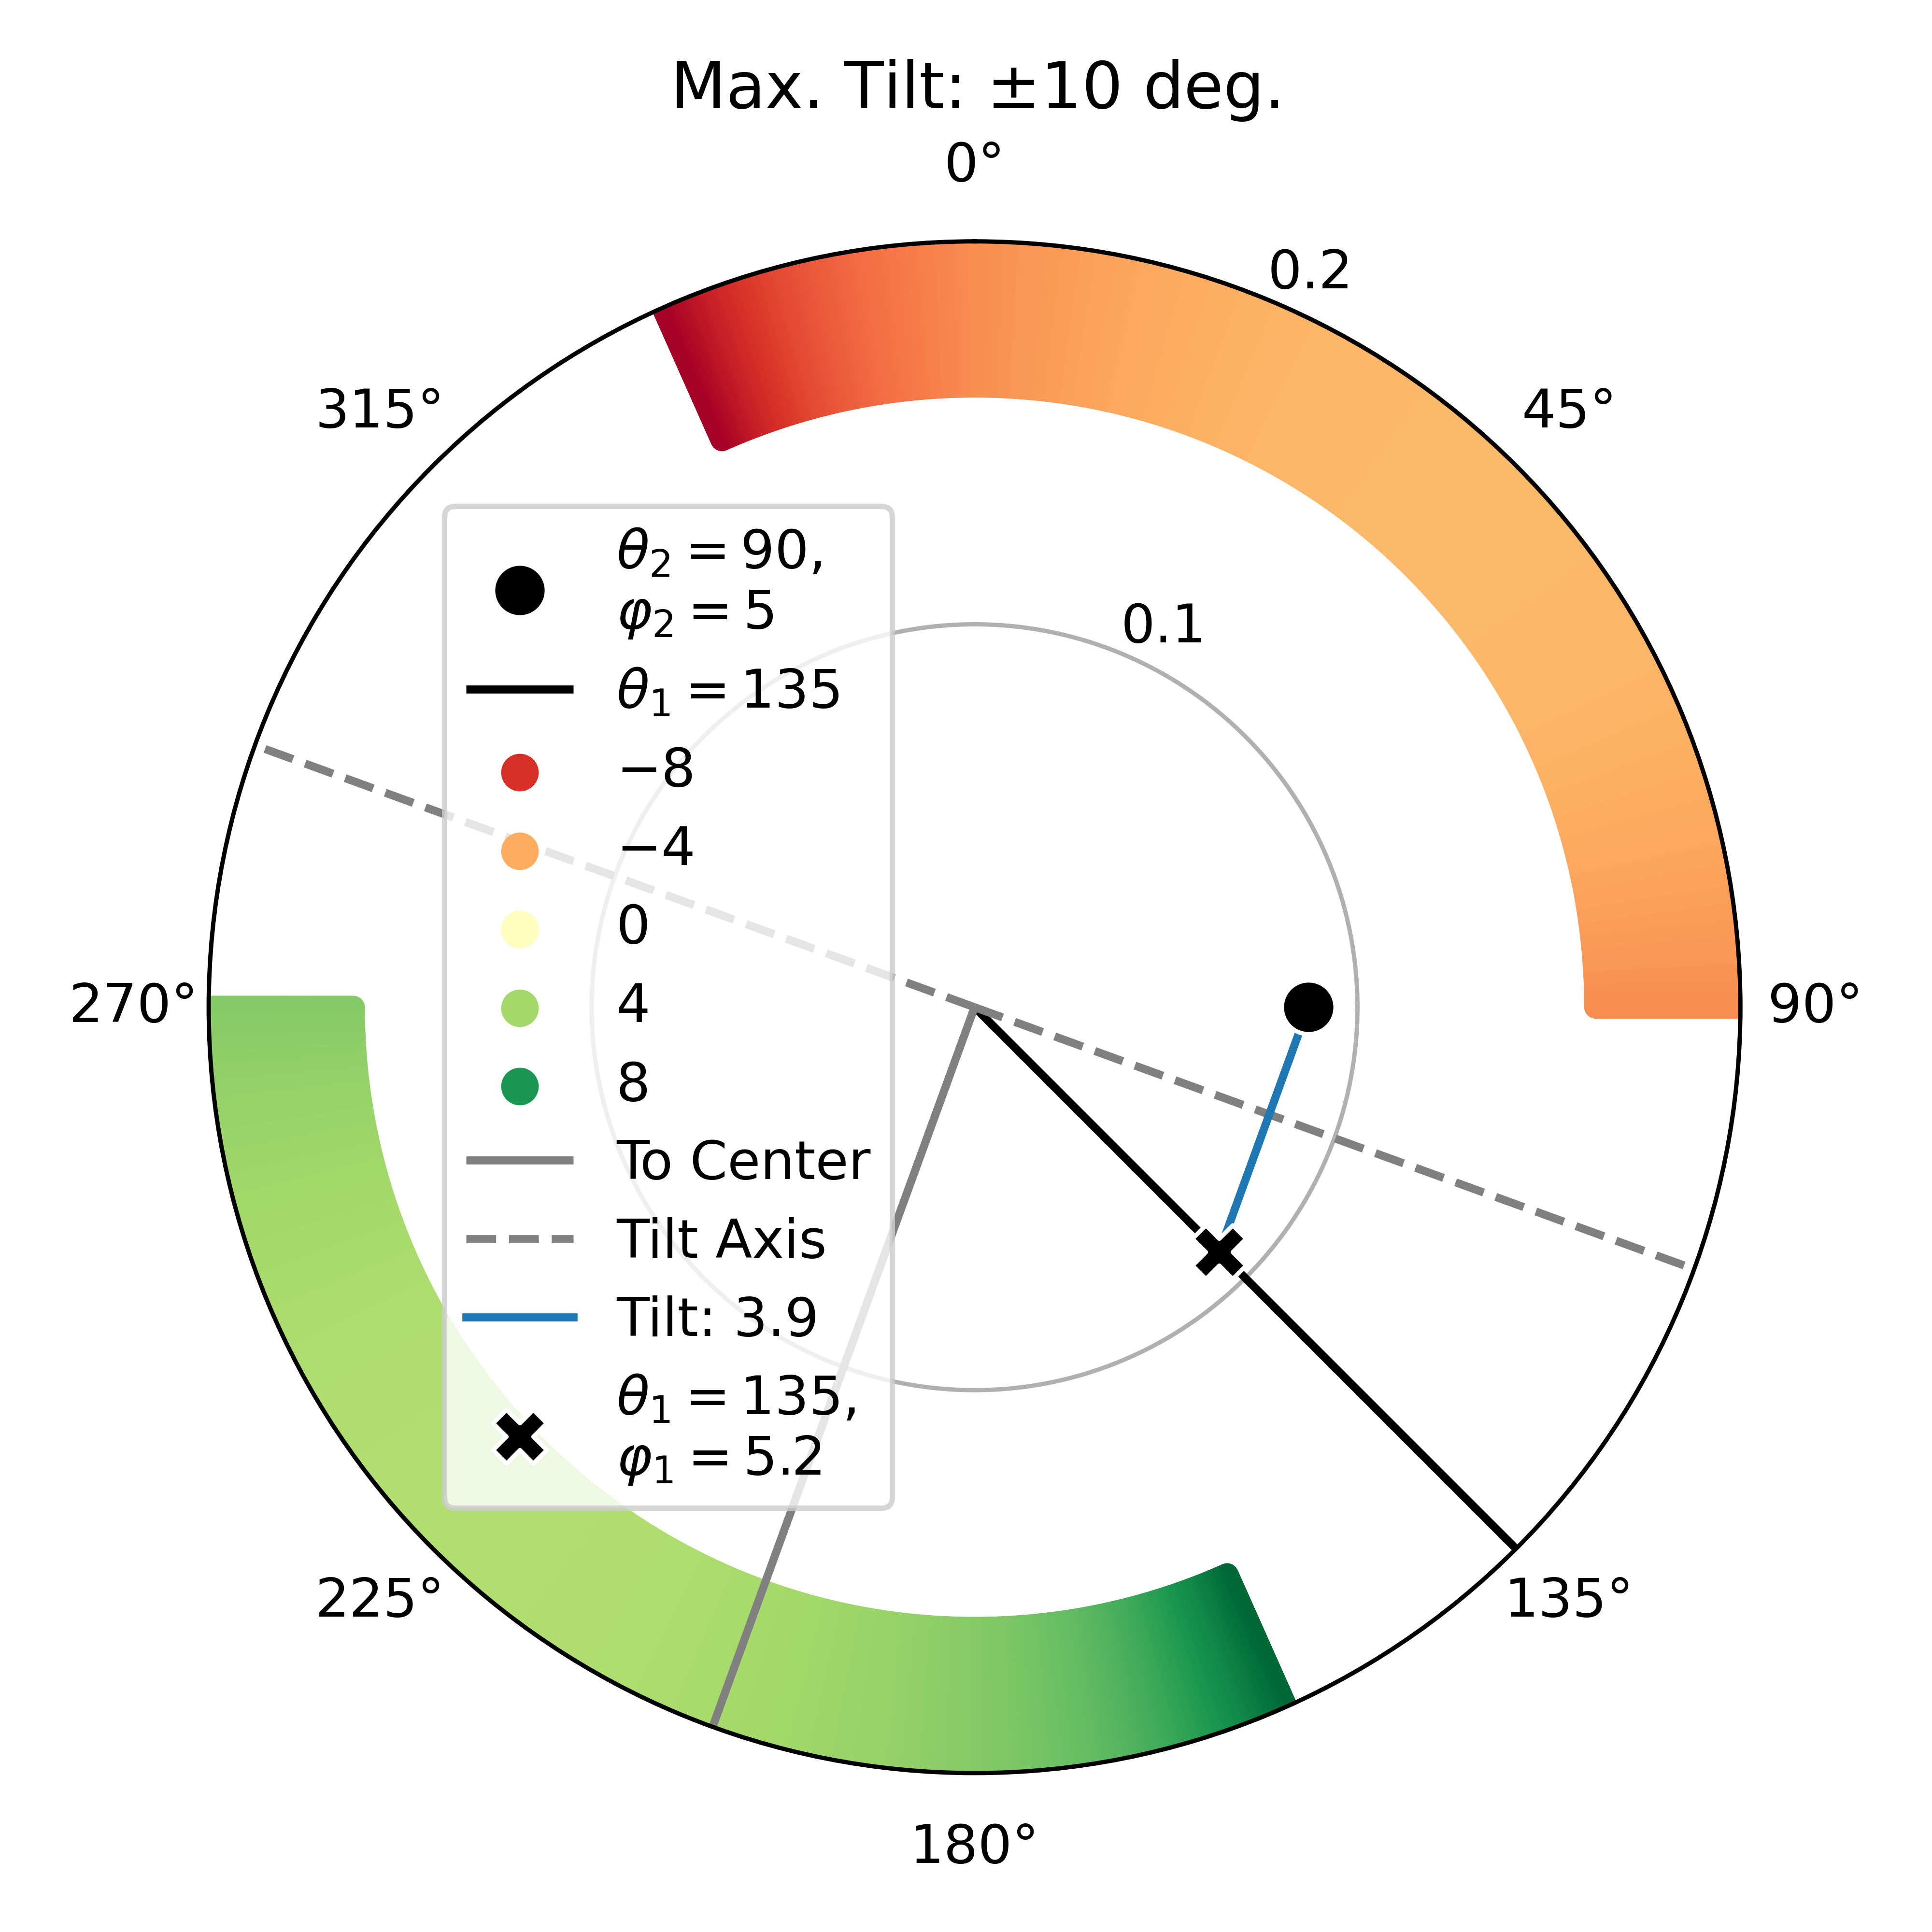
\includegraphics[width=.5\textwidth]{methods/tilt-check-example-rim.png}%
    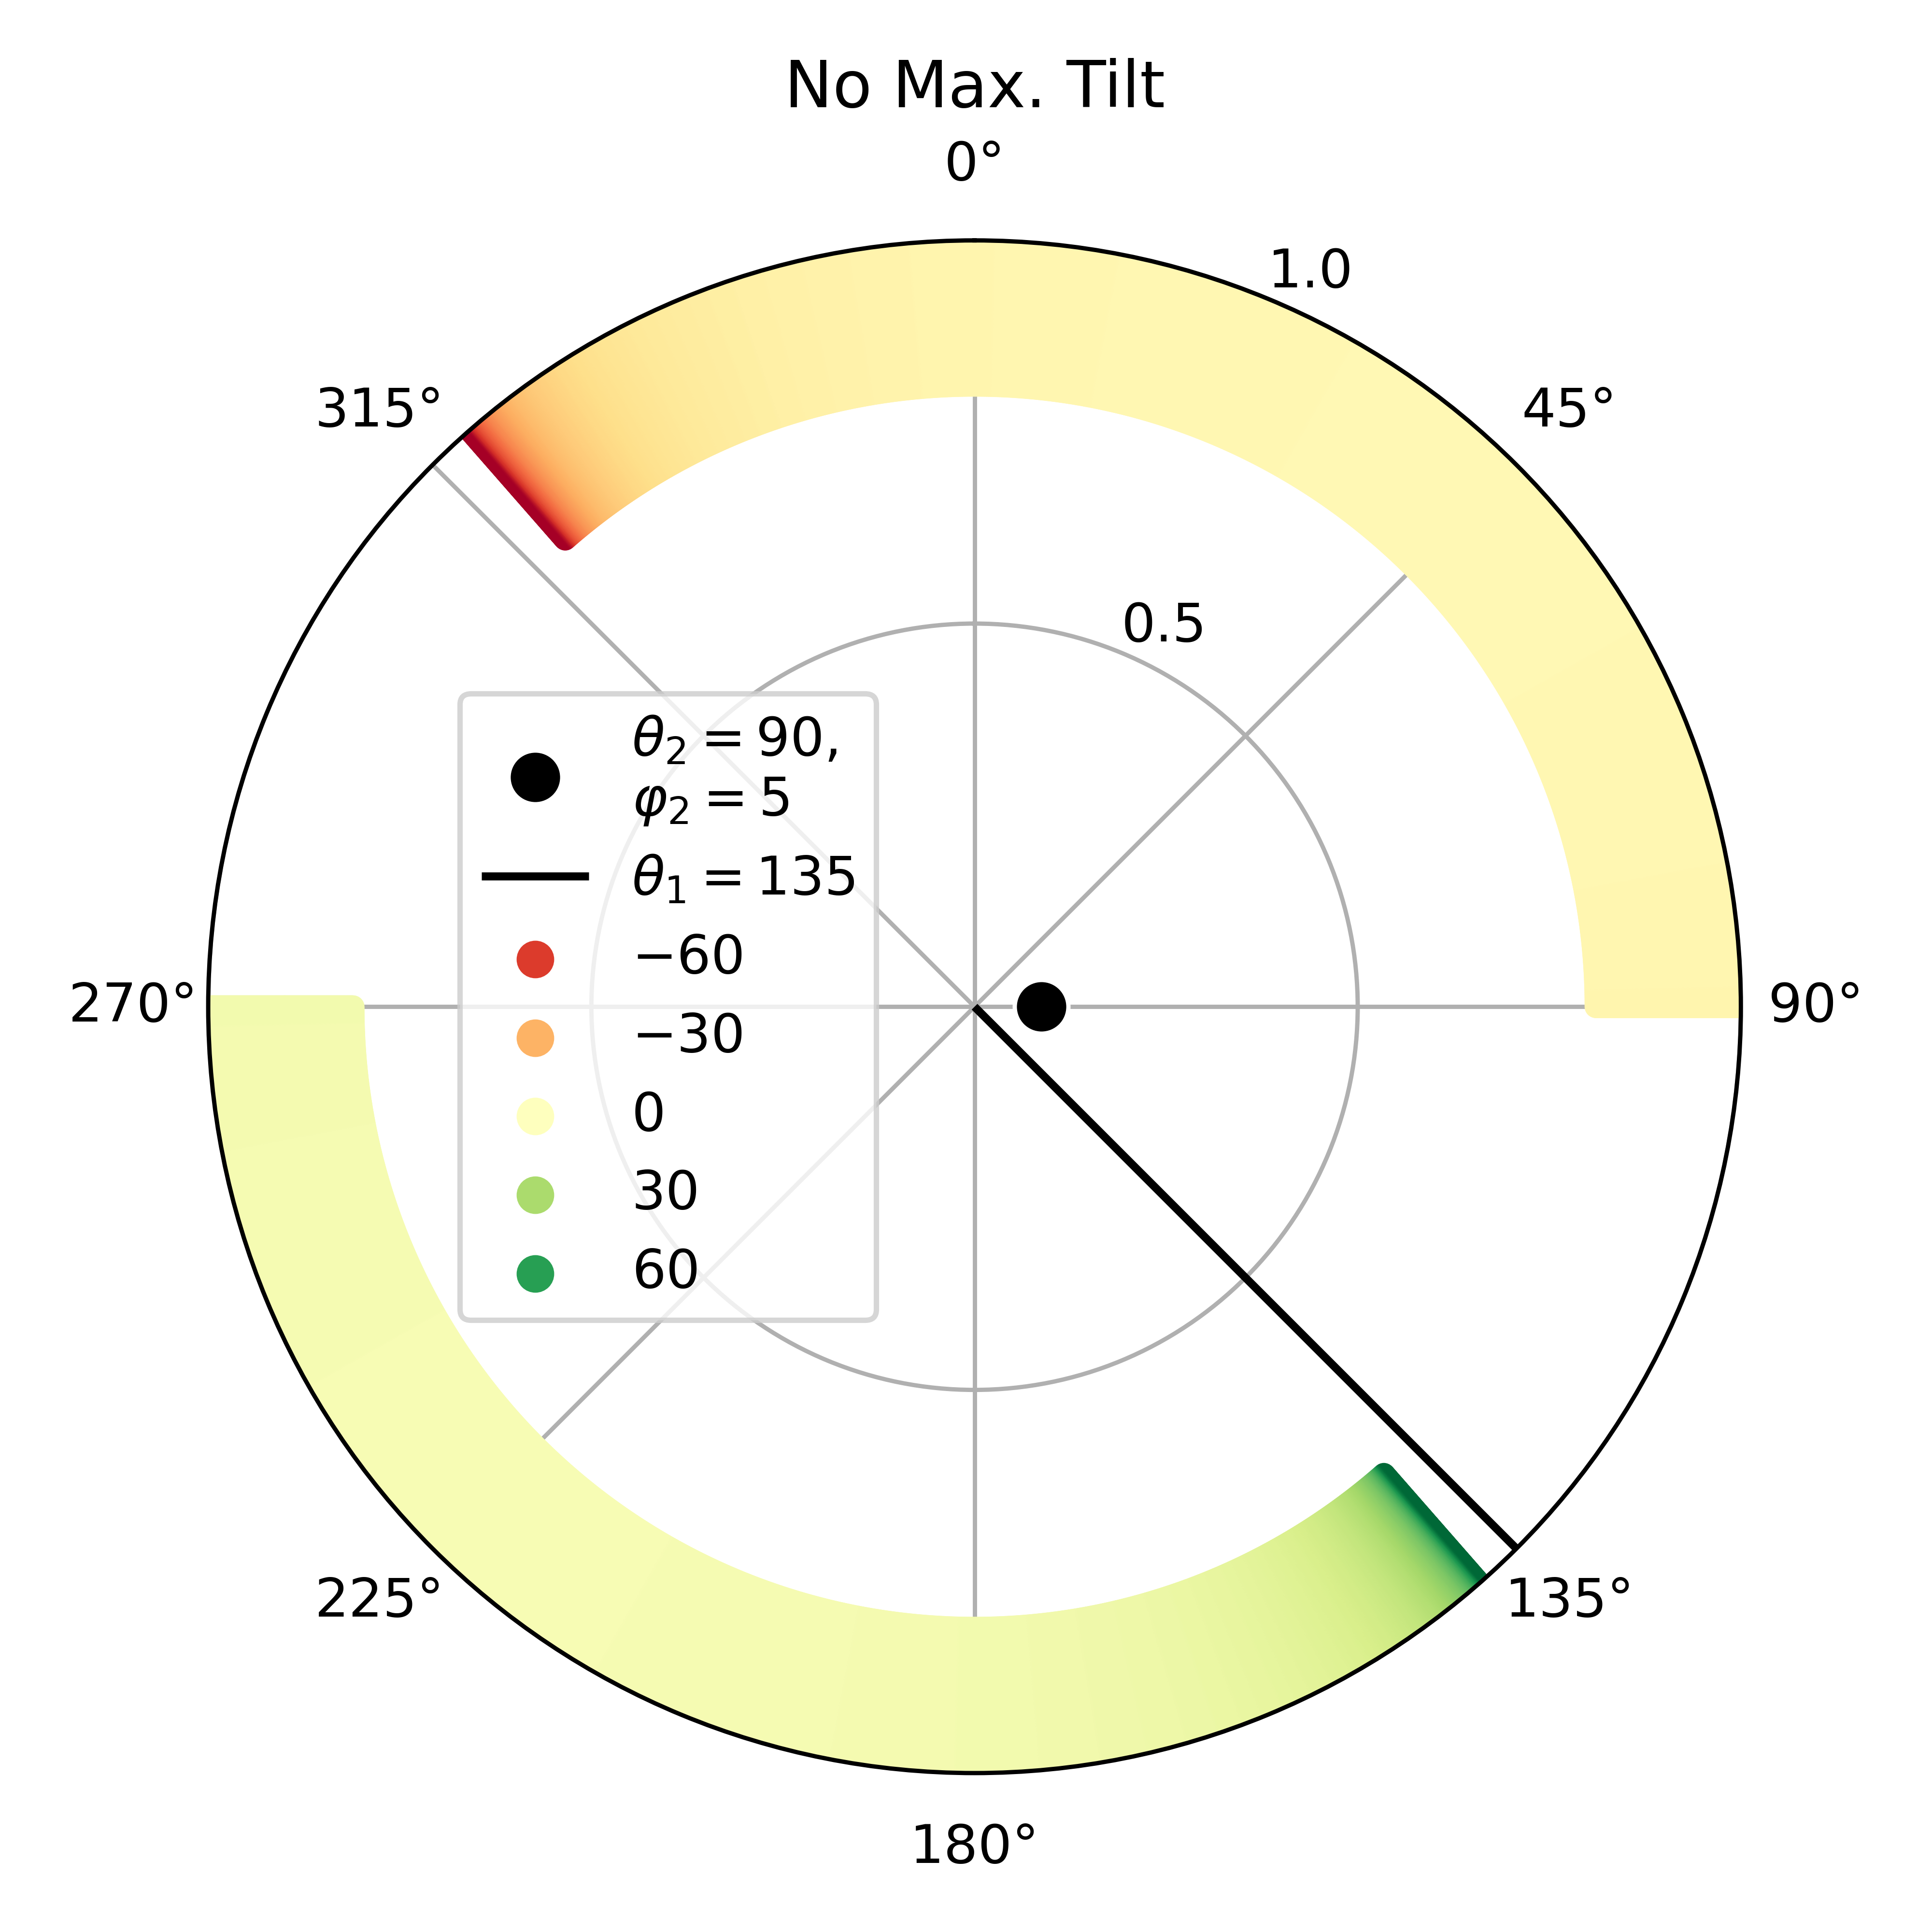
\includegraphics[width=.5\textwidth]{methods/tilt-check-rim.png}%
    \caption[Tilt calculation example]{Tilt calculation (Equation~\ref{eq:tilt-from-map}) example. \textbf{Top Left:} A discordant feature in an upper hemisphere orthographic projection, as in Figure~\ref{fig:attitude-data}. \textbf{Top Right:} A candidate inflation center to the SSW (North is \ang{0}) implies \ang{+3.9} degrees of tilt about the dashed tilt axis to sweep a paleo-attitude ($\times$) across the blue tilt-path to reach the modern attitude. Note the tilt path is perpendicular to the tilt axis and parallel to the center direction, as in Figure~\ref{fig:tilt-from-map}. \textbf{Bottom Left:} Tilt calculation repeated for all ``directions to center'' and assigned a color on the appropriate rim location. For example, the SSW center line intersects the light green color matching \ang{3.9} of tilt. Tilts exceeding \ang{10} excluded here to highlight variation. \textbf{Bottom Right:} Example removed for clarity. Tilts exceeding \ang{10} included.}
    \label{fig:tilt-example}
\end{figure}

% \begin{figure}
%     \vspace{-19pt}
%     \includegraphics[width=.5\textwidth]{methods/tilt-behavior-high-max.pdf}%
%     \includegraphics[width=.5\textwidth]{methods/tilt-behavior-non-discordant.pdf}\\
%     \includegraphics[width=.5\textwidth]{methods/tilt-behavior-opposite.pdf}%
%     \includegraphics[width=.5\textwidth]{methods/tilt-behavior-opposite-high-uncertainty.pdf}%
%     \caption[Tilt calculation behavior]{Tilt calculation behavior under a variety of circumstances. \textbf{Top Left:} Full range of center directions for the example geometry in Figure~\ref{fig:tilt-example}. Note that a) necessary tilt increases rapidly as center direction approaches the feature orientation (in Figure~\ref{fig:tilt-from-map}, as $\acs{beta1}\to\ang{0}$ or $\acs{beta1}\to\pm\ang{180}$) and b) some orientations are impossible, as discussed in Section~\ref{sec:paleo-slope}. \textbf{Top Right:} Non-discordant features ($\acs{disc} < \ang{7}$) cannot imply non-zero tilt in any orientation. \textbf{Bottom Left:} The most discordant features ($\acs{disc}\approx\pm\ang{180}$; flows point directly uphill) imply a narrow range of tilt orientations. \textbf{Bottom Right:} Possible tilt configurations for highly discordant features are strongly influenced by the choice of \acs{az1}-uncertainty (compare with bottom left).}
%     \label{fig:tilt-behavior}
% \end{figure}

The final product of this section is a transformation from mapped attitude data (Figure~\ref{fig:attitude-data}) at a particular location $(\acs{lat}, \acs{lon})$ to a tilt-distance data point corresponding to a single inflation center candidate $(\acs{latC}, \acs{lonC})$. Figure~\ref{fig:tilt-example} illustrates the final results. Repeating the tilt and distance calculations for each sample (within a discordant population of interest) to produce a full tilt-distance dataset corresponding to a single center candidate. Finally, repeating this dataset construction for each center allows the full array of candidates to be evaluated and compared.